% Template for Elsevier
% version 1.1-5p dated 18 January 2011
% NO ACCENTUATION PROBLEM UTF-8 : NOT ACCEPTED

% This file (c) 2010-2011 Elsevier Ltd. Modifications may be freely made,
% provided the edited file is saved under a different name

% This file contains modifications for Procedia Computer Science
% but may easily be adapted to other journals


%-----------------------------------------------------------------------------------

%% This template uses the elsarticle.cls document class and the extension package ecrc.sty
%% For full documentation on usage of elsarticle.cls, consult the documentation "elsdoc.pdf"
%% Further resources available at http://www.elsevier.com/latex

%-----------------------------------------------------------------------------------

%%%%%%%%%%%%%%%%%%%%%%%%%%%%%%%%%%%%%%%%%%%%%%
%%%%%%%%%%%%%%%%%%%%%%%%%%%%%%%%%%%%%%%%%%%%%%
%%                                          %%
%% Important note on usage                  %%
%% -----------------------                  %%
%% This file must be compiled with PDFLaTeX %%
%% Using standard LaTeX will not work!      %%
%%                                          %%
%%%%%%%%%%%%%%%%%%%%%%%%%%%%%%%%%%%%%%%%%%%%%%
%%%%%%%%%%%%%%%%%%%%%%%%%%%%%%%%%%%%%%%%%%%%%%

%% The '5p' and 'times' class options of elsarticle are used for Elsevier CRC
\documentclass[5p]{elsarticle}


%%%%%%%%%%%%%%%%%%%%%%%%%%%%%%%%% 
\usepackage[english]{babel}     % Language
\usepackage{float}
\usepackage[latin1]{inputenc}   % Latin-1 encoding
\usepackage{amsmath}             % For equation references with \eqref
\usepackage{flushend}            % To equalize columns on the last page
\usepackage[colorlinks=true,linkcolor=blue,citecolor=blue,urlcolor=blue]{hyperref}
\newcommand*{\doi}[1]{\href{http://doi.org/#1}{#1}}

%%%%%%%%%%%%%%%%%%%%%%%%%%%%%%%%%%%%%%%%%%%%%%%%%%%%%%%

%% Hereafter the template follows `elsarticle'.
%% For more details see the existing template files elsarticle-template-harv.tex and elsarticle-template-num.tex.

%% Elsevier CRC generally uses a numbered reference style
%% For this, the conventions of elsarticle-template-num.tex should be followed (included below)
%% If using BibTeX, use the style file elsarticle-num.bst

%%%%%%%%%%%%%%%%%%%%%%%%%%%%%%%%%%%%%%%%%%%%%%%%%%%%%%%%%%%%%%%%%%%%%%%%%%

%% The amssymb package provides various useful mathematical symbols
\usepackage{amssymb}
%% The amsthm package provides extended theorem environments
%% \usepackage{amsthm}

%% The lineno packages adds line numbers. Start line numbering with
%% \begin{linenumbers}, end it with \end{linenumbers}. Or switch it on
%% for the whole article with \linenumbers after \end{frontmatter}.
%% \usepackage{lineno}

%% natbib.sty is loaded by default. However, natbib options can be
%% provided with \biboptions{...} command. Following options are
%% valid:

%%    round  -  round parentheses are used (default)
%%    square -  square brackets are used    [option]
%%    curly  -  curly braces are used      {option}
%%    angle  -  angle brackets are used    <option>
%%    semicolon  -  multiple citations separated by semi-colon
%%    colon  - same as semicolon, an earlier confusion
%%    comma  -  separated by comma
%%    numbers-  selects numerical citations
%%    super  -  numerical citations as superscripts
%%    sort   -  sorts multiple citations according to order in ref. list
%%    sort&compress    -  like sort, but also compresses numerical citations
%%    compress - compresses without sorting
%%
%% \biboptions{comma,round}


% if you have landscape tables
\usepackage[figuresright]{rotating}

% put your own definitions here:
%    \newcommand{\cZ}{\cal{Z}}
%    \newtheorem{def}{Definition}[section]
%    ...

% add words to TeX's hyphenation exception list
%\hyphenation{author another created financial paper re-commend-ed Post-Script}

% to be able to introduce multiple figures that occupy the width of the two columns.
\usepackage{subfigure}

% declarations for front matter

\begin{document}


\begin{frontmatter}
    

%% Title, authors and addresses

%% use the tnoteref command within \title for footnotes;
%% use the tnotetext command for the associated footnote;

%% use the fnref command within \author or \address for footnotes;
%% use the fntext command for the associated footnote;

%% use the corref command within \author or corresponding author footnotes;
%% use the cortext command for the associated footnote;
%% use the ead command for the email address,
%% and the form \ead[url] for the home page:
%%
%% \title{Title\tnoteref{label1}}
%% \tnotetext[label1]{}
%% \author{Name\corref{cor1}\fnref{label2}}
%% \ead{email address}
%% \ead[url]{home page}
%% \fntext[label2]{}
%% \cortext[cor1]{}
%% \address{Address\fnref{label3}}
%% \fntext[label3]{}

%\dochead{Article Header}
%% Use \dochead if there is an article header, e.g. \dochead{Short communication}

\title{Titulo aqui}


%% use optional labels to link authors explicitly to addresses:
%% \author[label1,label2]{<author name>}
%% \address[label1]{<address>}
%% \address[label2]{<address>}

\author[First]{Nombre y Apellidos\corref{cor1}}
\ead{correo@unsa.edu.pe}
\ead[url]{https://orcid.org/XXXX-XXXX-XXXX-XXXX}

\author[First]{Nombre y Apellidos\corref{cor1}}
\ead{correo@unsa.edu.pe}
\ead[url]{https://orcid.org/XXXX-XXXX-XXXX-XXXX}

\author[First]{Nombre y Apellidos\corref{cor1}}
\ead{correo@unsa.edu.pe}
\ead[url]{https://orcid.org/XXXX-XXXX-XXXX-XXXX}

\author[First]{Nombre y Apellidos\corref{cor1}}
\ead{correo@unsa.edu.pe}
\ead[url]{https://orcid.org/XXXX-XXXX-XXXX-XXXX}

\author[First]{Nombre y Apellidos\corref{cor1}}
\ead{correo@unsa.edu.pe}
\ead[url]{https://orcid.org/XXXX-XXXX-XXXX-XXXX}

%%COMENTADO\fntext[label2]{Footnote for author 1}
\cortext[cor1]{Corresponding author.}

%% DIRECCIÓN COMENTADO
\address[First]{Universidad Nacional de San Agust{\'i}n, Arequipa, Per{\'u}.}
%%

\begin{abstract}
%% Text of abstract
Resumen aqui.
\end{abstract}

\begin{keyword}
%% keywords here, in the form: keyword \sep keyword

%% MSC codes here, in the form: \MSC code \sep code
%% or \MSC[2008] code \sep code (2000 is the default)

Palabras clave 1 \sep Palabra clave 2 \sep Palabra clave 3 \sep Palabra clave 4 \sep Palabra clave 5.
\end{keyword}


%%
%% Start line numbering here if you want
%%
% \linenumbers
\end{frontmatter}


%% main text
\section{Introduction}
\label{sec:introduction}
Introduccion .....

\section{Related Work}
\label{sec:related_work}
Trabajos relacionados .....

\section{Material and Methods}
\label{sec:material_methods}

\subsection{Theoretical background}
\label{sec:theoretical_background}
Fundamentos teoricos .....

\subsection{Tools and technologies}
\label{sec:tools_technologies}
Herramientas y tecnologias .......

Tabla a 2 columnas
\begin{table*}[htbp]
  \caption{Titulo descriptivo de la tabla ancha.}
  \label{tab:table1}
  \centering
  \begin{tabular}{p{0.25\textwidth} p{0.25\textwidth} p{0.25\textwidth} p{0.2\textwidth}}
   \hline
    \textbf{Parameter} & \textbf{Description} & \textbf{Description} & \textbf{Description} \\
    \hline
    Parameter1 & Text of example. & Text of example. & Text of example. \\
    Parameter2 & Text of example. & Text of example. & Text of example. \\
    Parameter3 & Text of example. & Text of example. & Text of example. \\
    Parameter4 & Text of example. & Text of example. & Text of example. \\
    \hline
  \end{tabular}
\end{table*}

\subsection{Dataset}
\label{sec:dataset}
Dataset ....

Ejemplo de ecuacion
\begin{equation}
\mathit{F1\text{-}score} = 2 \times \frac{\mathit{Precision} \times \mathit{Recall}}{\mathit{Precision} + \mathit{Recall}}
\label{eq:eq1}
\end{equation}

\subsection{Proposed methodology}
\label{sec:proposed_methodology}
Metodologia propuesta


Ejemplo de Figura a dos columnas.

\begin{figure*}[tb]
\centerline{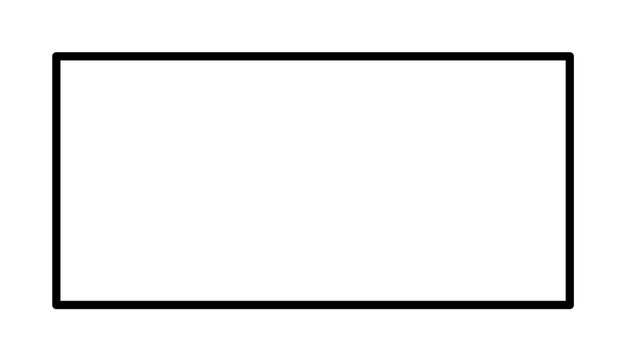
\includegraphics[width=2\columnwidth]{images/img1.jpg}}
\caption{Figure example}
\label{fig:fig1}
\end{figure*}

\section{Results}
\label{sec:results}
Resultados

Ejemplo de Figura a una columna.
\begin{figure}[H]
\centerline{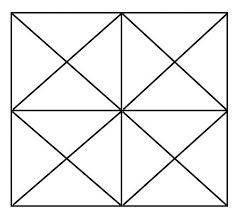
\includegraphics[width=1\columnwidth]{images/img2.png}}
\caption{Figure example}
\label{fig:fig2}
\end{figure}

\section{Discussion}
\label{sec:discussion}
Discusion

Ejemplo de Tabla a una columna

\begin{table}[H]
  \centering
  \caption{Ejemplo de Tabla}
  \label{tab:table2}
  \begin{tabular*}{\hsize}{l p{4cm}}
    \hline
    \textbf{Parameter} & \textbf{Description} \\
    \hline
    Parameter1 & Text of example. \\
    Parameter2 & Text of example. \\
    Parameter3 & Text of example. \\
    Parameter4 & Text of example. \\
    \hline
  \end{tabular*}
\end{table}

\section{Conclusions}
\label{sec:conclusions}
Conclusiones

\section{Limitations and future work}
\label{sec:limitations_future_work}
Limitaciones y Trabajos Futuros \cite{wikipedia1}.

\section*{CRediT authorship contribution statement}
\label{sec:authorship_contribution}
Contribucion de cada autor segun los roles Credit

\section*{Declaration of competing interest}
\label{sec:competing_interest}
The authors declare that they have no known competing financial interests or personal relationships that could have appeared to influence the work reported in this paper.

\section*{Ethical statement}
\label{sec:ethical_statement}
This study does not involve any experiments on humans or animals, and no ethical approval was required. Therefore, an ethical statement is not applicable.

\section*{Consent to participate}
\label{sec:consent_participate}
Not Applicable.

\section*{Consent for publication}
\label{sec:consent_publication}
Not Applicable.

\section*{Funding}
\label{sec:funding}
Not Applicable.

\section*{Acknowledgement}
\label{sec:acknowledgement}
Not Applicable.

\section*{Code availability}
\label{sec:code_availability}
The custom analysis scripts and source code generated during this study are publicly available in [Repository Name] at doi: \doi{10.123456/987654}, licensed under a [License Name, e.g., MIT License].

\section*{Data availability}
\label{sec:data_availability}
The data supporting this study's findings are available in Kaggle at url: \url{https://www.google.com.pe}.

%% References with BibTeX database:

\bibliographystyle{elsarticle-num}
\bibliography{references}

\end{document}